\title{Study Guide 2 for Algebra-Based Physics-1: Mechanics (PHYS135A-01)}
\author{Dr. Jordan Hanson - Whittier College Dept. of Physics and Astronomy}
\date{October 24th, 2018}
\documentclass[10pt]{article}
\usepackage[a4paper, total={18cm, 27cm}]{geometry}
\usepackage{outlines}
\usepackage[sfdefault]{FiraSans}
\usepackage{graphicx}
\usepackage{amsmath}

\begin{document}
\maketitle

\section{Equations}
\begin{itemize}
\item Newton's First Law: $\vec{F}_{Net} = 0$ if $\vec{v}$ is constant.  Newton's Second Law: $\vec{F}_{Net} = m \vec{a}$. Newton's Third Law: $\vec{F}_{AB} = -\vec{F}_{BA}$.
\item Normal force: $\vec{N} = +mg\hat{y}$, if weight is $w = -mg\hat{y}$ (flat surface).
\item Force of Friction: $\vec{F} = -\mu \vec{N}$ (minus sign: opposes motion).
\item Static versus kinetic friction: $\mu_s \geq \mu_k$.
\item Definition of velocity: $\vec{v} = \frac{\Delta \vec{x}}{\Delta t}$
\item Definition of acceleration: $\vec{a} = \frac{\Delta \vec{v}}{\Delta t}$
\item Constant acceleration: 
\begin{enumerate}
\item $v(t) = at + v_i$
\item $x(t) = \frac{1}{2} a t^2 + v_i t + x_i$
\item $v^2 = v_i^2 + 2 a \Delta x$
\end{enumerate}
\end{itemize}

\section{Newton's Laws}
\begin{enumerate}
\small
\item An swimmer sinks at constant velocity to the bottom of the ocean near the shore.  The swimmer has a weight force downwards.  In which direction is there another force on the swimmer?
\begin{itemize}
\item A: \textbf{Upwards.} - Newton's first law.
\item B: Downwards.
\item C: Towards the shore.
\item D: Away from shore.
\end{itemize}
\item A soccer player in training begins to sprint down the field.  She has a mass $m$, is wearing a harness than has mass $M$, and has acceleration $a$.  If she exerts constant force through her cleats on the turf, and drops the harness, which of the following is true?
\begin{itemize}
\item A: Her new acceleration will be less than $a$.
\item B: \textbf{Her new acceleration will be greater than $a$.} - Newton's second law.
\item C: Her new acceleration will be equal to $a$.
\item D: Her new acceleration will be 0.
\end{itemize}
\item Consider Fig. \ref{fig:fbd1}.  Which of the following is true regarding the system in the diagram?
\begin{itemize}
\item A: It has no net force.
\item B: It is accelerating to the left.
\item C: \textbf{It is accelerating to the right.} - Newton's second law.  The vector pointing to the left is not a force.
\item D: It is accelerating downwards. 
\end{itemize}
\begin{figure}[h]
\centering
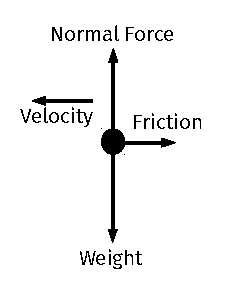
\includegraphics[width=0.15\textwidth]{figures/FBD3.pdf}
\caption{\label{fig:fbd1} A free body diagram for a system.}
\end{figure}
\item Consider Fig. \ref{fig:fbd1}.  Suppose the system reaches a point where there is no longer friction.  Which of the following is true?
\begin{itemize}
\item A: \textbf{The system will move at a constant velocity.} - Newton's second law.  The vertical vectors will cancel and $F_{net}$ will be zero.
\item B: The system will accelerate to the right.
\item C: The system will stop moving.
\item D: The system will accelerate to the left.
\end{itemize}
\item A 70 kg sprinter begins a run at rest and reaches 10 m/s in 3.0 seconds.  What force does he exert on the track? \\ \\
The acceleration is needed to compute the force.  \textbf{Using the \textit{definition of acceleration}, we have $a = (10-0)/(3.0-0.0) = 10/3$ m/s$^2$. Knowing the acceleration, we can use Newton's second law $F = (70)(10/3) = 233$ N.}
\item Consider Fig. \ref{fig:sled}, in which two children pull their friend on a sled resting on snow with forces $\vec{F}_1$ and $\vec{F}_2$.  (a) What is the magnitude of the net force (no friction)? (b) If sled and the child on it have total mass 40 kg, what is the acceleration? \\ \\ 
\textbf{(a) To obtain the magnitude of the net force, we first must add the force vectors to obtain the net force.  Let $\theta_1$ and $\theta_2$ be the corresponding angles.} \\
\begin{align}
F_{1x} &= F_1 \cos\theta_1 \\
F_{2x} &= F_2 \cos\theta_2 \\
F_{1y} &= F_1 \sin\theta_1 \\
F_{2y} &= F_2 \sin\theta_2
\end{align}
\textbf{Add the vectors to get the net force: $\vec{F}_{net} = (F_1 \cos\theta_1+F_2 \cos\theta_2,F_1\sin\theta_1+F_2 \sin\theta_2)$.  Plugging in numbers, we obtain $F_{net} = (7.07+6.93,7.07-4.0) = (14,3.07)$ N. Use the Pythagorean theorem to obtain the magnitude $\sqrt{14^2+3.07^2} = 14.3$ N.  (b) Knowing the net force, we can obtain the acceleration $a = F_{net}/m = 14.3/40 = 0.36$ m/s$^2$.}
\begin{figure}[h]
\centering
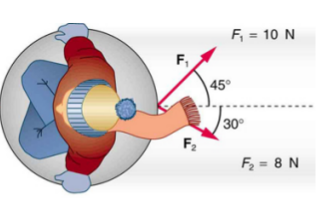
\includegraphics[width=0.4\textwidth]{figures/sled.png}
\caption{\label{fig:sled} Two children pull a third on a sled.}
\end{figure}
\item A 20,000 kg jet pushes through the air with a forward force of $10^6$ N, and faces air resistance equivalent to $5 \times 10^4$ N.  What is the acceleration of the jet? \\ \\
\textbf{We need the net force to obtain the acceleration: $F_{net} = 10^6- 5\times 10^4$ N.  The acceleration is $ F_{net}/m = (10^6- 5\times 10^4)/(2\times 10^4 = \frac{100}{2} - \frac{5}{2} = 47.5$ m/s$^2$.  This is the equivalent of $47.5/9.8 = 4.8$ g's.}
\end{enumerate}
\section{Friction and Drag}
\small
\begin{enumerate}
\item A woman drags a piece of luggage across a floor.  If the mass of the luggage is 30 kg, and she exerts a force of 300 N, what is the coefficient of kinetic friction between the luggage and floor? \\ \\
Let's just assume $g=10$, and we have the normal force $N$ is $mg \approx 30\times 10 = 300$ N.  The frictional force is $\mu N$, so $F_{lady} = \mu m g$, or $\mu = 1.0$.  (This assumes the luggage is being dragged at constant velocity).
\item Consult Fig. \ref{fig:coeff}. (a) What is the magnitude of the force of friction exerted on an oiled steel piston experiencing a normal force of 10 N from another steel surface? (b) What would the result have been if the steel had no oil? \\ \\
\textbf{The frictional force is just $\mu N$, and according to the table, $\mu_k = 0.03$, so $0.03 \times 10$ N, which is 0.3 N.  If there is no oil, $\mu_k = 0.3$, so the friction would be 3 N.}
\begin{figure}
\centering
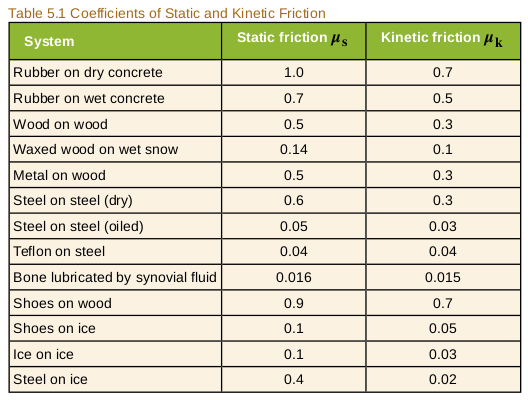
\includegraphics[width=0.55\textwidth]{figures/coefficients.png}
\caption{\label{fig:coeff} (Left) Frictional coefficients for exercise 2, \textbf{Friction and Drag}.}
\end{figure}
\item Consult Fig. \ref{fig:blocks}.  Recall the lab in which we measured the coefficient of static friction, $\mu_s$.  If $\mu_s = 0.5$, and $m_2=200$ grams, what is the smallest mass $m_1$ can be before the system begins to accelerate? \\ \\
\textbf{If the system is static, then the net force is zero (Newton's first law).  The weight creates tension which balances the frictional force (just as we saw in the lab activity). $F_f = T$.  Thus, $\mu_s m_1 g = m_2 g$, so $m_1 = m_2/\mu_s = 200/0.5 = 400$ grams.  If $m_1$ were \textit{smaller}, the system would accelerate because it would overcome static friction.}
\begin{figure}[hb]
\centering
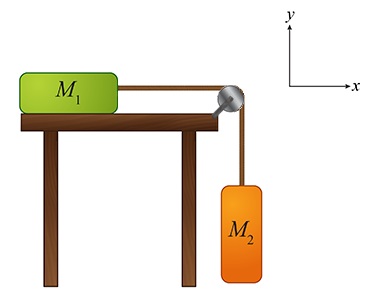
\includegraphics[width=0.25\textwidth]{figures/table.png}
\caption{\label{fig:blocks} Diagram for exercise 3, \textbf{Friction and Drag}.}
\end{figure}
\item A system travels at a \textit{terminal velocity} $v_{T} = \sqrt{2mg/C\rho A}$.  (a) What is $v_{T}$ for a falling system who with $m=200$ kg, $A=2$ m$^2$, $C \approx 0.4$, in air with $\rho_{air}=1.225$ kg/m$^3$? (See section 5.3 of the textbook). \\ \\ 
Plug and chug: $v_T = \sqrt{2*200*10/(4/10)/1.225/2} \approx 64$ m/s.
\end{enumerate}
\end{document}